% TODO replace by long version
\begin{figure}
  \centering
  \begin{tikzpicture}    
    %\node at (-3.5,0) {
    %  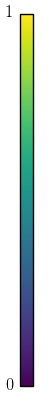
\includegraphics[height=5cm]{experiments/3d/vae_occ_sdf/colorbar_0}
    %};
    
    \node at (0, 1.2){
      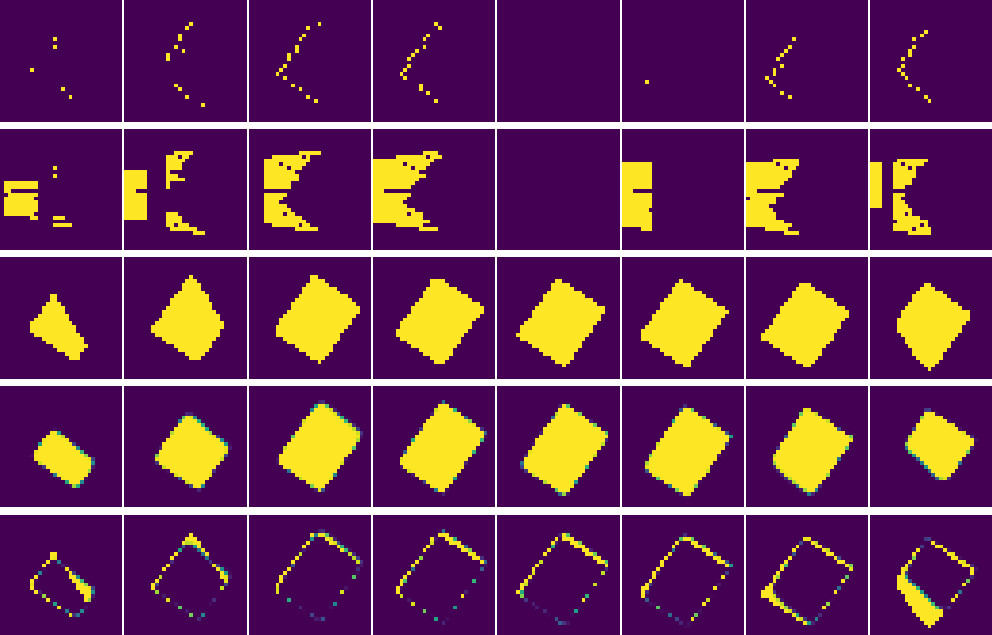
\includegraphics[width=6cm]{experiments/shapenet/vae_occ/easy_15_long/results_1}
    };
    \node at (0, -1.2){
      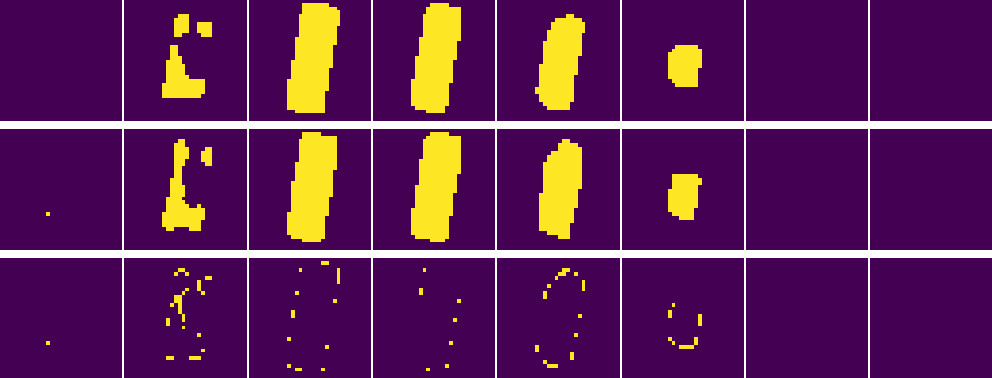
\includegraphics[width=6cm]{experiments/shapenet/vae_occ/easy_15_long/results_2}
    };
    
    \node at (6.5, 0){
      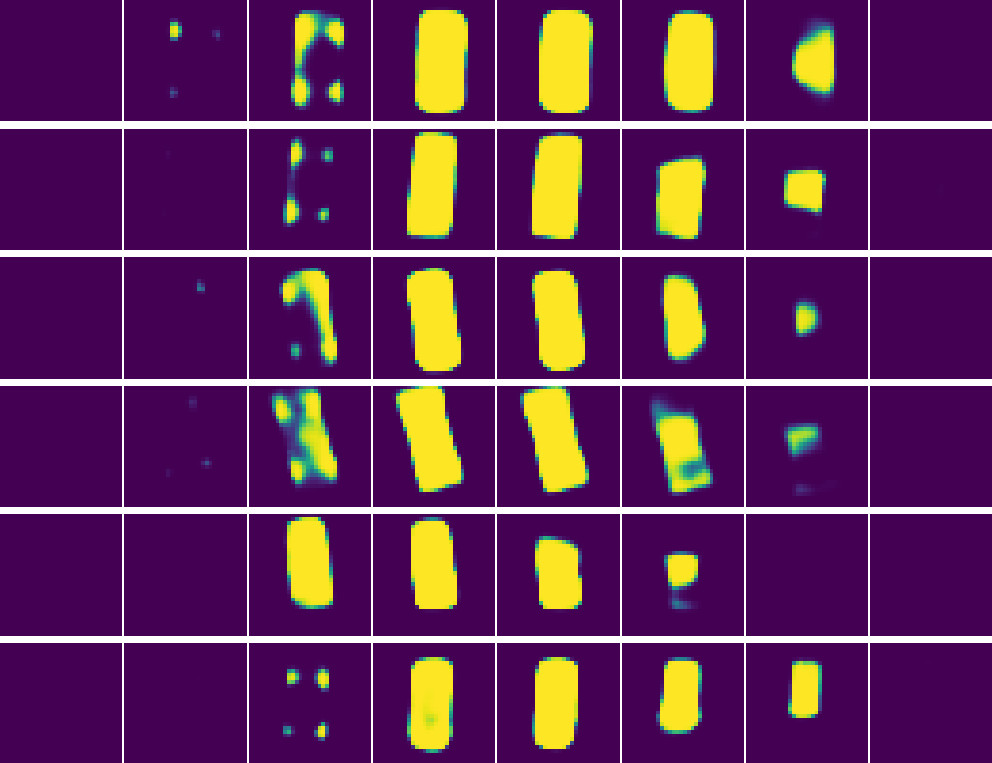
\includegraphics[width=6cm]{experiments/shapenet/vae_occ/easy_15_long/random_0}
    };
    
    \node at (0, 3) {\begin{tabular}{c}reconstruction\\occupancy\end{tabular}};
    \node at (6.5, 3) {\begin{tabular}{c}random samples\\occupancy\end{tabular}};
    
    \draw[-,dashed] (-3.5, -2.5) -- (10, -2.5);
    
    \node at (10, 0) {
      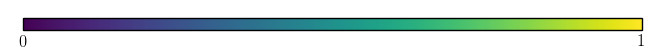
\includegraphics[height=4.2cm]{experiments/3d/vae_occ/easy_15/colorbar}
    };
    
    %\node at (-3.5,-5) {
    %  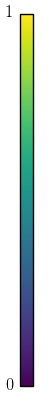
\includegraphics[height=5cm]{experiments/3d/vae_occ_sdf/colorbar_0}
    %};
    
    \node at (0, -5){
      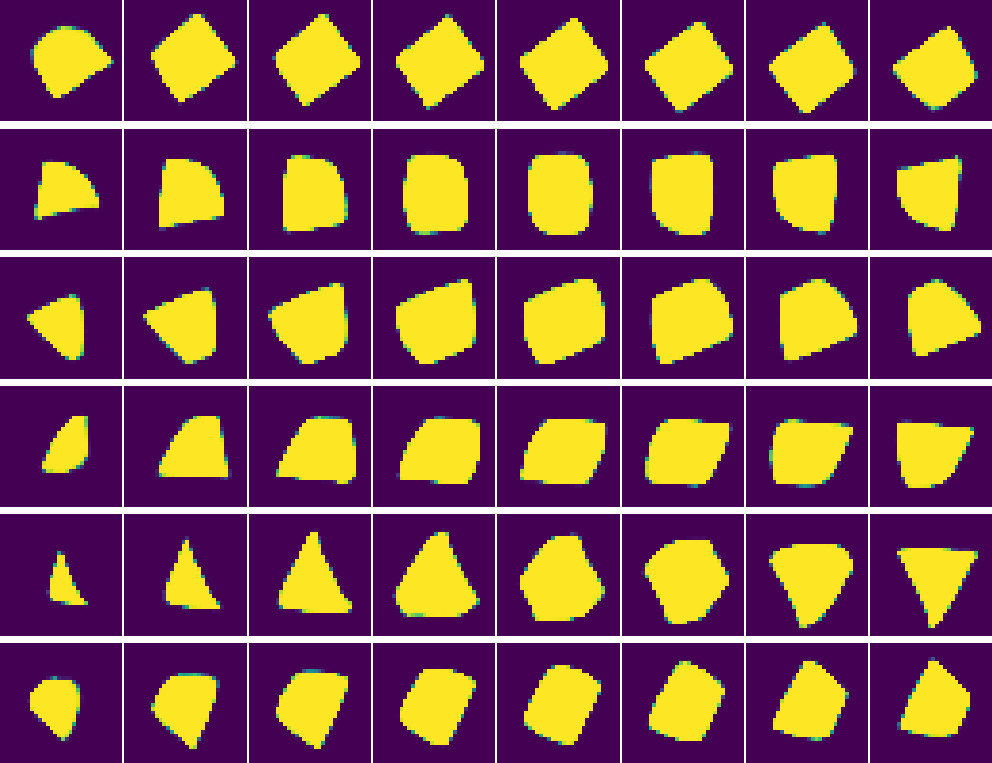
\includegraphics[width=6cm]{experiments/shapenet/vae_occ_sdf/easy_15/random_0_0}
    };
    
    %\draw[-,dashed] (3.25, -3) -- (3.25,3);
    
    \node at (6.5, -5){
      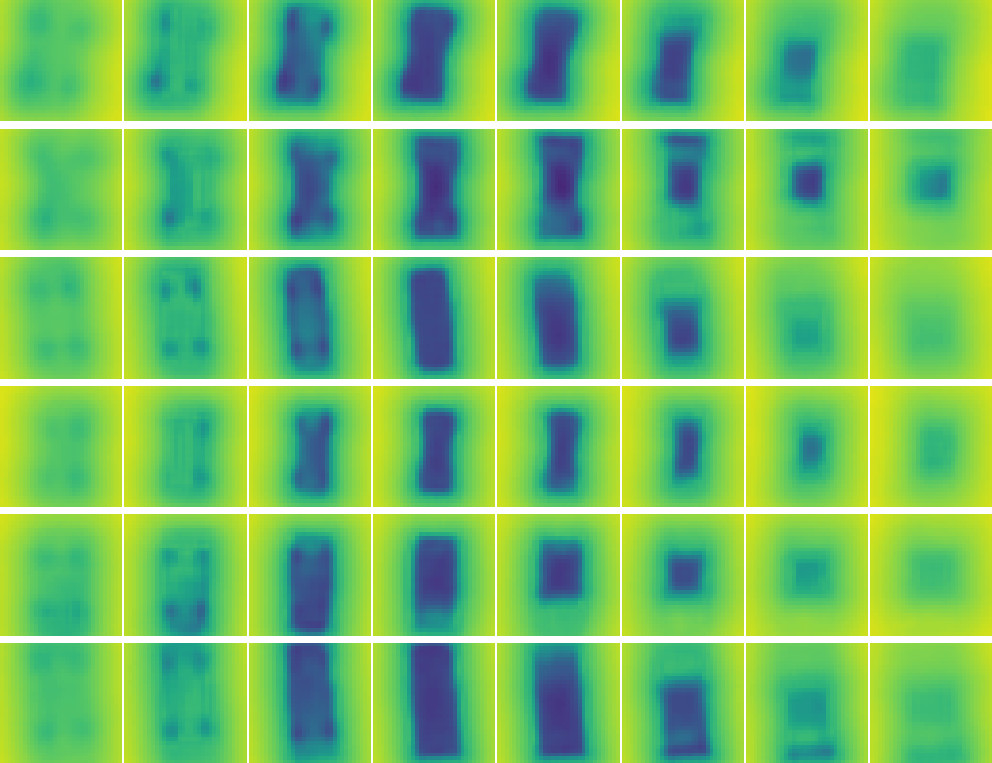
\includegraphics[width=6cm]{experiments/shapenet/vae_occ_sdf/easy_15/random_0_1}
    };
    
    \node at (10,-5) {
      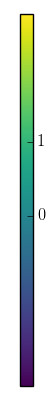
\includegraphics[height=5cm]{experiments/3d/vae_occ_sdf/colorbar_1}
    };
    
    \node[rotate=90] at (-3.75, 0) {\begin{tabular}{c}predicting occupancy only\end{tabular}};
    \node[rotate=90] at (-3.75, -5) {\begin{tabular}{c}predicting occupancy and\\signed distance functions\end{tabular}};
        
    \node at (0, -8) {\begin{tabular}{c}random samples\\occupancy\end{tabular}};
    \node at (6.5, -8) {\begin{tabular}{c}random samples\\signed distance functions\end{tabular}};
  \end{tikzpicture}
  \caption{Qualitative results considering reconstruction and random samples
  for a \VAE prior, $Q = 15$, learned on ShapeNet using occupancy only (top) and
  both occupancy and signed distance functions. In the latter case we only show
  random samples in both modalities. For reconstructions we show the target shape,
  the prediction as well as the corresponding error. In all cases we resort to
  showing horizontal slices as done before. 3D visualizations
  of the random samples can be found in Figures \ref{fig:experiments-shapenet-vae-qual-2}
  and \ref{fig:experiments-shapenet-vae-qual-3}.}
  \label{fig:experiments-shapenet-vae-qual-1}
\end{figure}
\begin{figure}
  \centering
  \hspace*{-0.75cm}
  \begin{tikzpicture}
    \node at (0, 0) {
      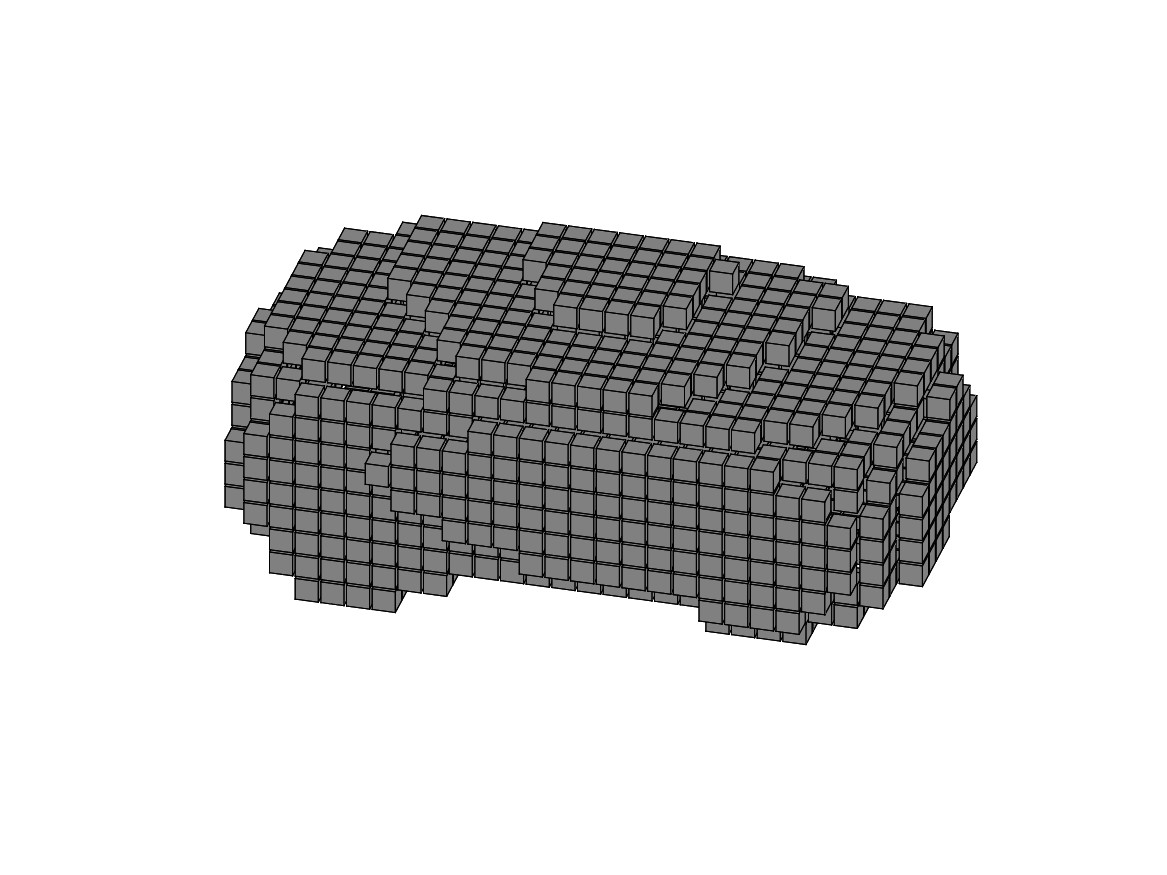
\includegraphics[width=2.5cm,trim={2cm 1cm 2cm 1cm},clip]{experiments/shapenet/vae_occ/easy_15_long/0_random_15}
    };
    \node at (2.5, 0) {
      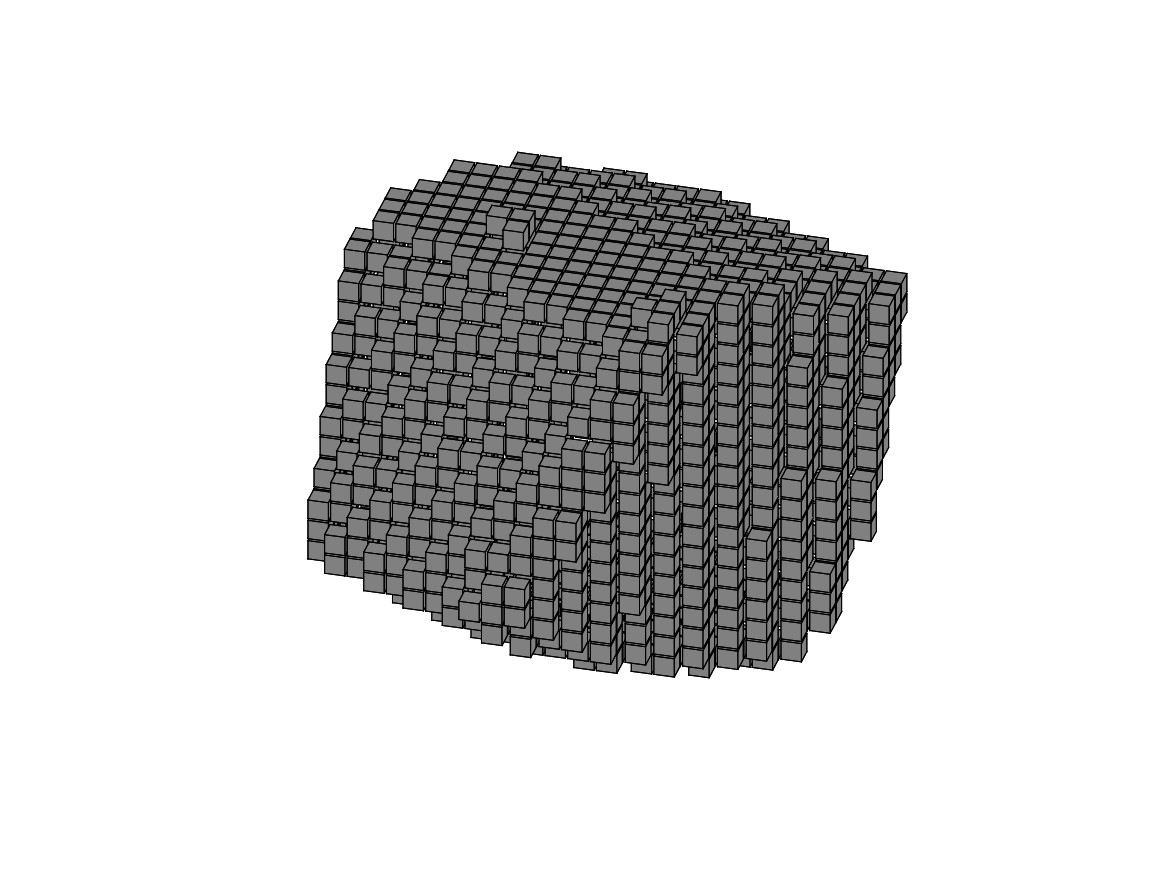
\includegraphics[width=2.5cm,trim={2cm 1cm 2cm 1cm},clip]{experiments/shapenet/vae_occ/easy_15_long/0_random_105}
    };
    
    \draw[-,dashed] (4,-1.5) -- (4, 1.5);
    
    \node at (5.5, 0) {
      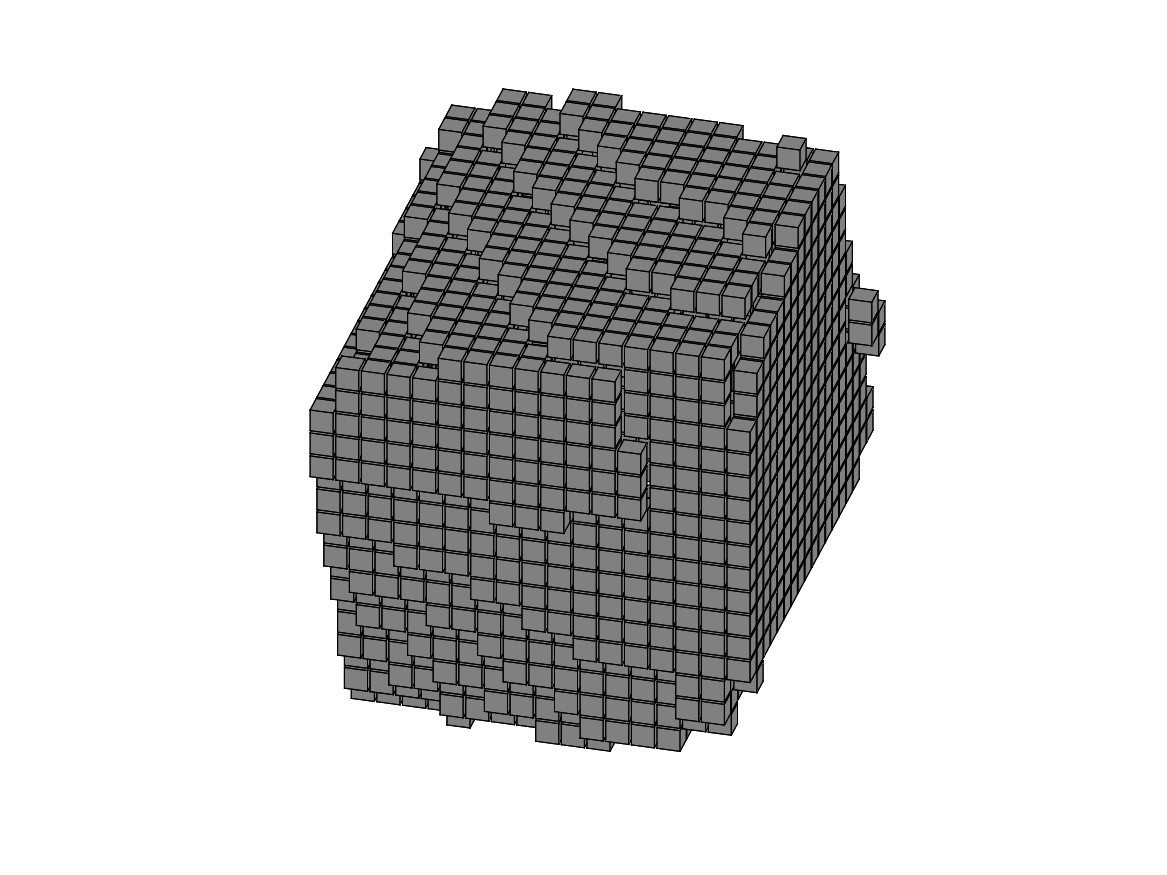
\includegraphics[width=2.5cm,trim={2cm 1cm 2cm 1cm},clip]{experiments/shapenet/vae_occ/easy_15_long/5_random_15}
    };
    \node at (8, 0) {
      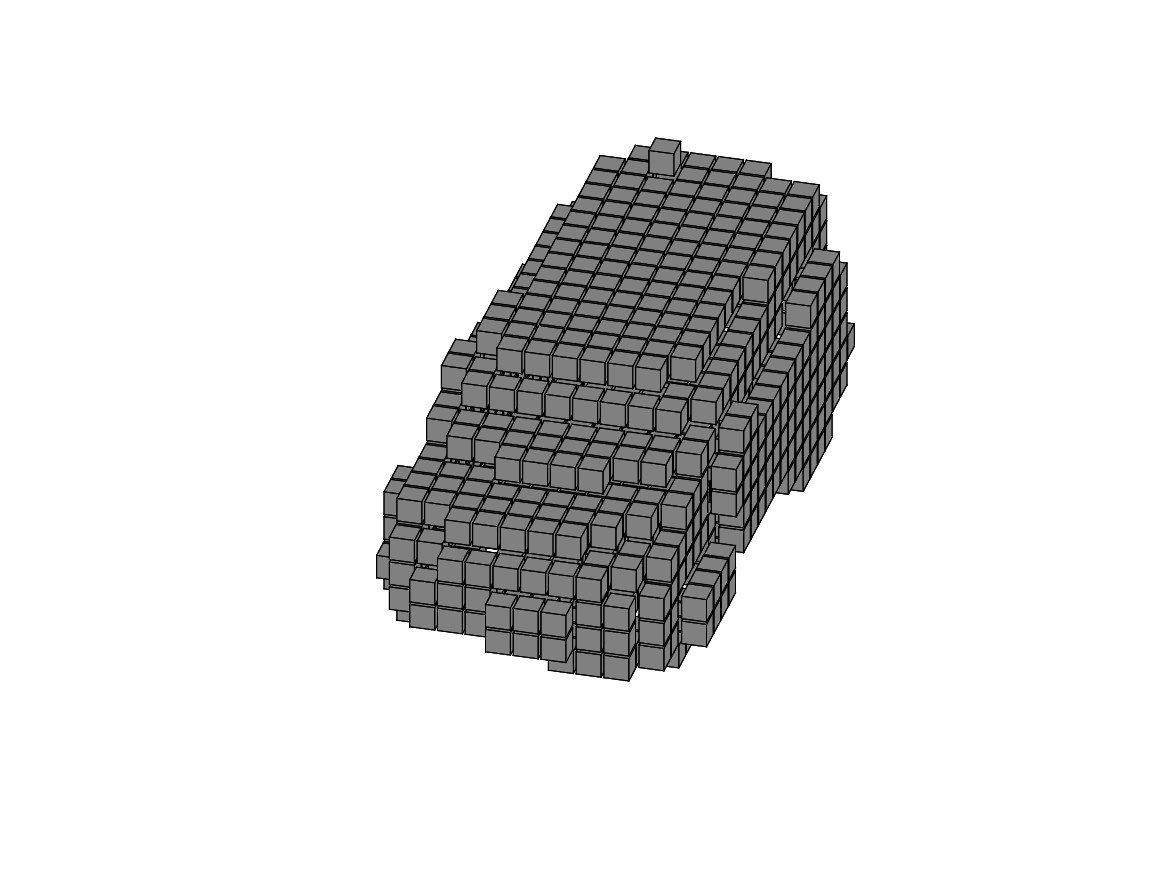
\includegraphics[width=2.5cm,trim={2cm 1cm 2cm 1cm},clip]{experiments/shapenet/vae_occ/easy_15_long/5_random_105}
    };
    
    \draw[-,dashed] (9.5,-1.5) -- (9.5, 1.5);
    
    \node at (11, 0) {
      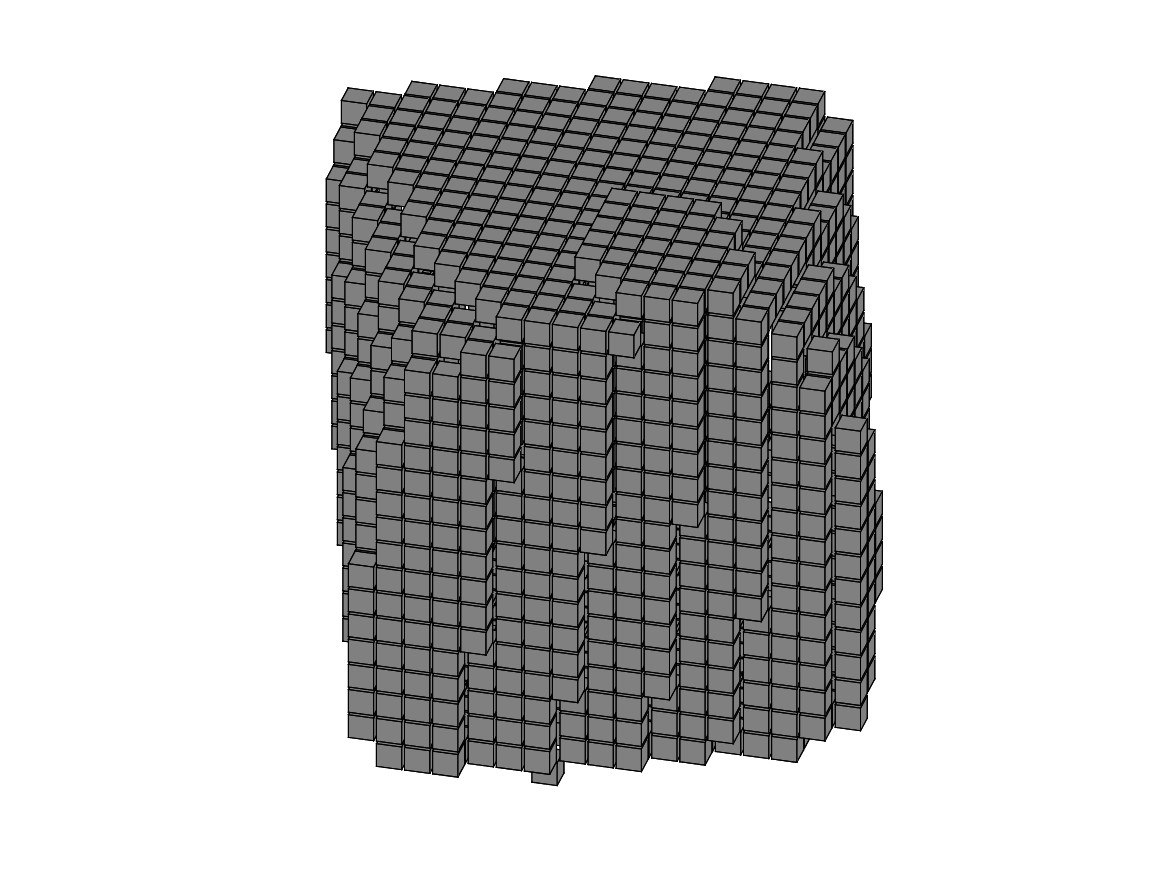
\includegraphics[width=2.5cm,trim={2cm 1cm 2cm 1cm},clip]{experiments/shapenet/vae_occ/easy_15_long/2_random_15}
    };
    \node at (13.5, 0) {
      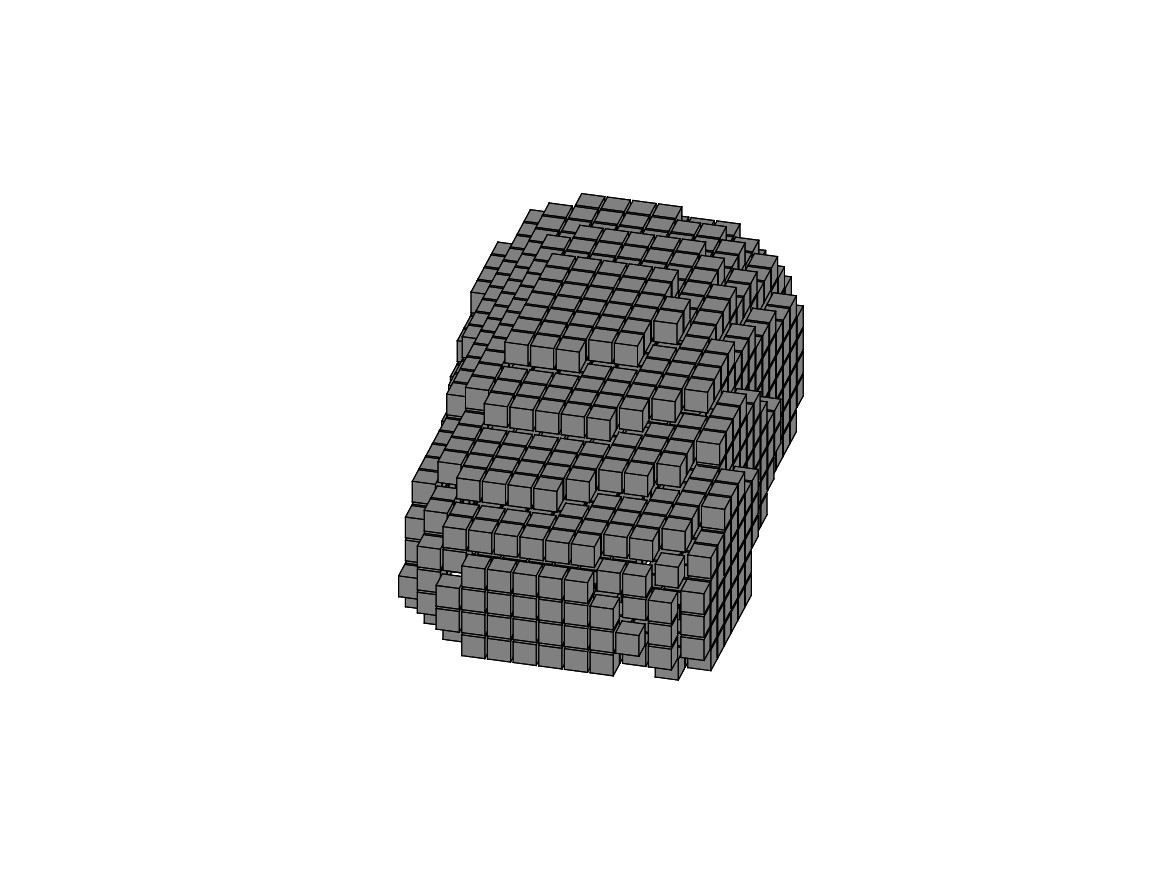
\includegraphics[width=2.5cm,trim={2cm 1cm 2cm 1cm},clip]{experiments/shapenet/vae_occ/easy_15_long/2_random_105}
    };
  \end{tikzpicture}
  \caption{3D visualizations of random samples obtained from a \VAE prior
  trained with $Q = 15$ and occupancy only on the ShapeNet dataset. We show three
  distinct samples using two viewpoints each. The samples
  can easily be recognized as cars, although details seem to be missing. However,
  this is also due to the low resolution of $32^3$ used.}
  \label{fig:experiments-shapenet-vae-qual-2}
\end{figure}
\begin{figure}
  \centering
  \hspace*{-0.5cm}
  \begin{tikzpicture}   
    \node at (0, 0) {
      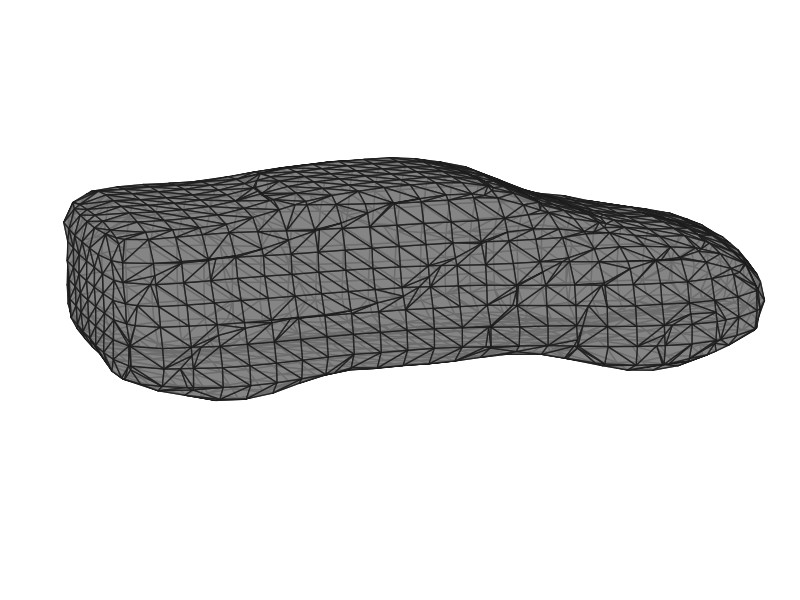
\includegraphics[width=2.4cm,trim={1cm 3cm 1cm 3cm},clip]{experiments/shapenet/vae_occ_sdf/easy_15/0_random}
    };
    
    \draw[-,dashed] (1.25,-1) -- (1.25, 1);
    
    \node at (2.5, 0) {
      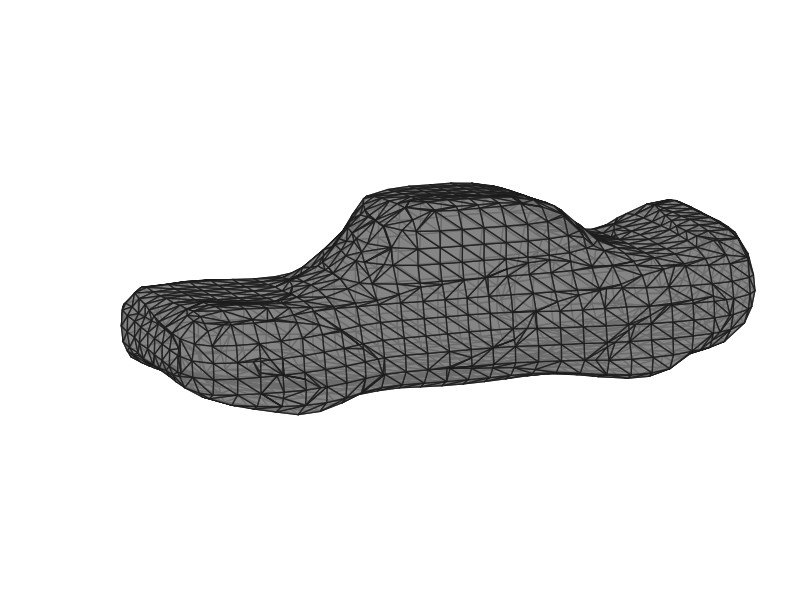
\includegraphics[width=2.4cm,trim={1cm 3cm 1cm 3cm},clip]{experiments/shapenet/vae_occ_sdf/easy_15/1_random}
    };
    
    \draw[-,dashed] (3.75,-1) -- (3.75, 1);
    
    \node at (5, 0) {
      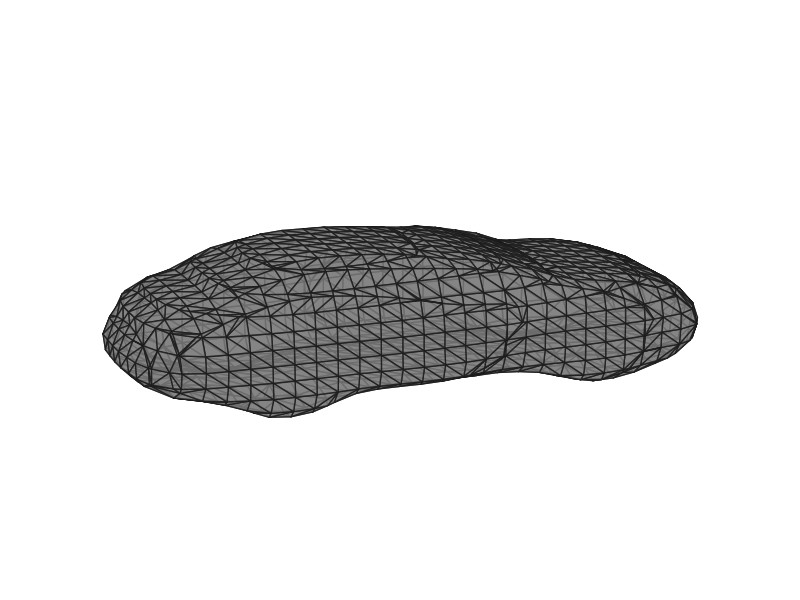
\includegraphics[width=2.4cm,trim={1cm 3cm 1cm 3cm},clip]{experiments/shapenet/vae_occ_sdf/easy_15/2_random}
    };
    
    \draw[-,dashed] (6.25,-1) -- (6.25, 1);
    
    \node at (7.5, 0) {
      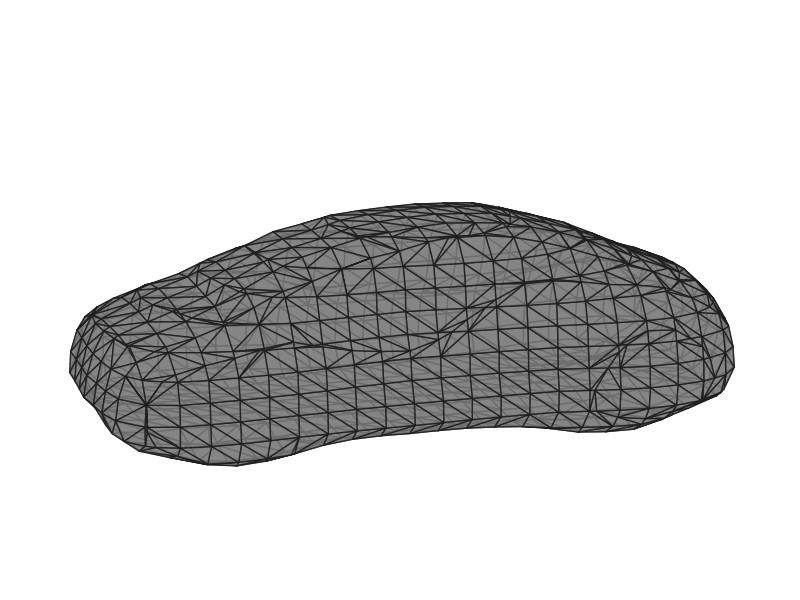
\includegraphics[width=2.4cm,trim={1cm 3cm 1cm 3cm},clip]{experiments/shapenet/vae_occ_sdf/easy_15/3_random}
    };
    
    \draw[-,dashed] (8.75,-1) -- (8.75, 1);
    
    \node at (10, 0) {
      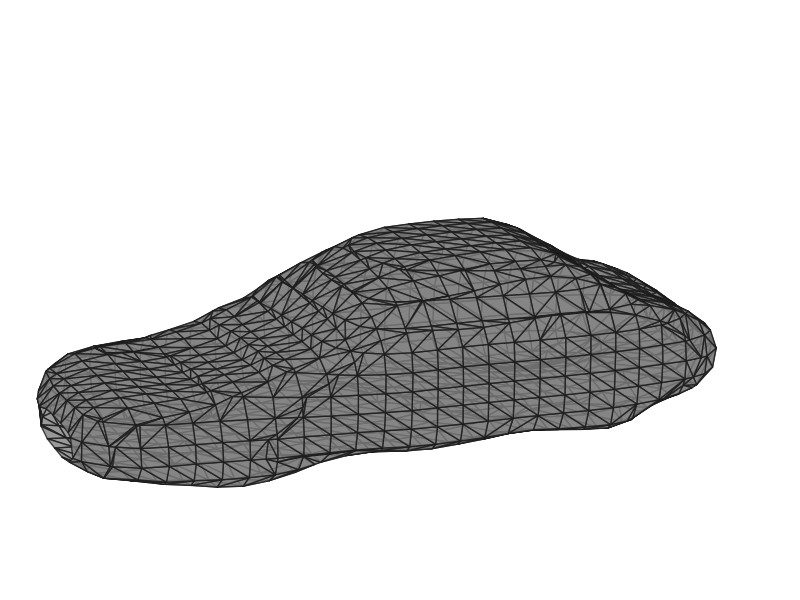
\includegraphics[width=2.4cm,trim={1cm 3cm 1cm 3cm},clip]{experiments/shapenet/vae_occ_sdf/easy_15/4_random}
    };
    
    \draw[-,dashed] (11.25,-1) -- (11.25, 1);
    
    \node at (12.5, 0) {
      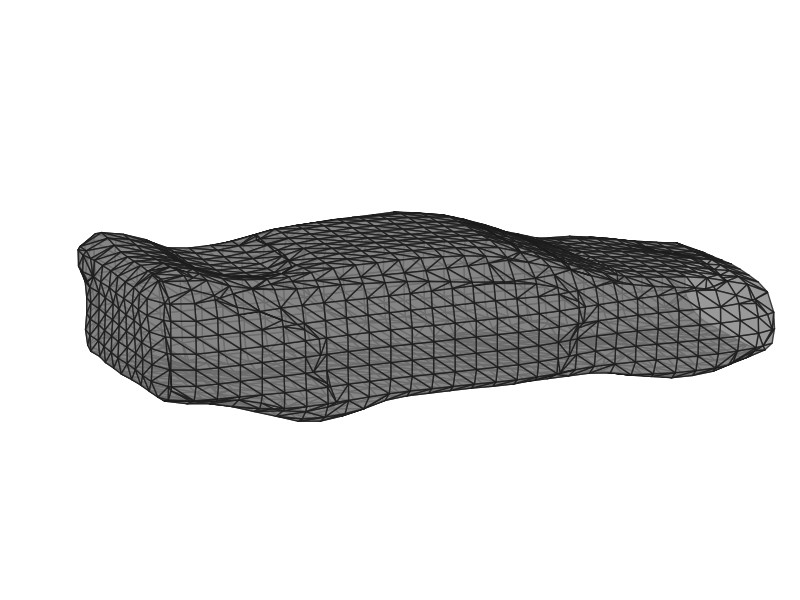
\includegraphics[width=2.4cm,trim={1cm 3cm 1cm 3cm},clip]{experiments/shapenet/vae_occ_sdf/easy_15/5_random}
    };
  \end{tikzpicture}
  \caption{3D visualizations of meshed random samples from a \VAE trained
  on both occupancy and signed distance functions. For meshing, we used the marching
  cubes algorithm on the predicted signed distance functions. We show a single viewpoint
  for each sample.}
  \label{fig:experiments-shapenet-vae-qual-3}
\end{figure}
